\chapter{Background} \label{chapter-background}

There are two great % #E MAYBE CHOOSE A MORE PRECISE WORD SUCH AS influential OR dominant
stories of \gls{distribution} in economics. The first and oldest is based on the classical concept of rent developed by Ricardo, in which owners of an asset are able to extract a value beyond what they contribute. 
The second is the marginalist approach, developed by Clark and others, in which workers receive the marginal value of their contribution to production. Both of these %accounts, frameworks, 
approaches were developed to explain how wealth is distributed. % across classes OR populations and both developed in response to the specific social and economic trends of the periods in which they emerged. 
% #E Distribution (ADD DISTRIBUTION TO GLOSSARY) , or how money OR resources OR wealth is allocated across class populations is an important idea in economic. Stories of distribution explain where wealth moves within  society and who captures the surplus, that is the excess wealth over and above WHAT.  %These accounts are, at their heart, stories of who claims what share of production. 
% #E FIRSTNAME Ricardo was a INSERT NATIONALITY classical economist  in the WHICH Century. Classical economics emerged in the 1600 and 1700 at a time of exploding colonial wealth and inequality. In this period, the COUNTRY economy was OR European economies were still structured largely around agricultural feudalism in which farmers OR peasants work the land that is owned by feudal aristocrats, but urban economies based around factories (AND ANYTHING ELSE)and colonial WHAT and trade routes...were just beginning to emerge as significant drivers of wealth. % #E Within this economic context, the surplus is captured by feudal aristocrats % through feudal mechanism of land ownership and flows into emerging town and city economies.
% ADD & EDIT : baroque urban excesses and Dickens children covered in tar and coal dying %95+
% The Classical Economics of this period was largely descriptive. 

As WHAT LED TO THE EXPLOSION... CHANGES IN UNIVERSITIES OR THE ECONOMY, there was an explosion of thinking about social and economic structures and systems.  This was a period where a range of thinkers explored many ideas to explain the shifting social and economic conditions. 

Distribution, or who got what share of production was a central concern. This focus came to the forefront in the 1600s and 1700s as colonial expansion of land holdings, factories and supplied change concentrated wealth- funding investment in the arts and sciences, great fortunes - harsher conditions for farmers, pushed of their land with enclosures, and concentrated in urban factories, almost exclusively poor with - illness bad working conditions % 90 rural,-- population snap shot % (unprecedented in northern Europe, a relative backwater) --  %gt (new ineuqlity- jusxtabosition- fortuioned unpreciendet ont hat content to rivla hsotori great- wons- woth workers dying, kids in factories- Dickens period, pesantry.. - both were new- the eilsure- )
 and concerned with inequality, which suited a time in which the labourers both on the land, and in the emerging factories struggled with poverty, at a time of rapidly growing -
-the intense interest spiked as wealth grew in colonial Europe. %(reformation another answer to this)
NOTABLY THIS WAS AN URBAN TRANSITION- FARMS TO SUBURBS- POWER GROWTH, AN INFLECTION - LIKE COVID REVEALED THE NEW FORM WITH A RAPID MOBILITY CHANGE..
The new form is the urban
dense exchange - experience in person density can compete with screen experience -

In this context, Ricardo developed the classical concept of rent.  % #E Today the word rent is usually used to refer to payments made by a tenant to a landlord to for the right to occupy a property, but this is not the traditional economic concept of  rent.  
% #E As a concept, it's more closely related to profit / surplus than to rent paid for properties. 
% #E NEED TO ADD HOW DOES THIS CONTRIBUTE OR EQUATE TO A THEORY OF DISTRIBUTION... WHAT DOES IT EXPLAIN...
Ricardo's concept of rent accounted for the way that.... WHAT IT DESCRIBED. 
This remains important to understanding distribution in general because.....

The second influential story of distribution is the marginalist approach, developed by Clark and others in the WHICH century. This account describes a distribution structure in which workers receive the marginal value of their contribution to production. THIS MEANS...

The marginalist account describes how workers receive the marginal value of their contribution to production. THIS MEANS.....
It formalizes what classical economist Adam Smith describes in the story of the pin factory. (EXPLAIN PIN FACTORY)

The marginalist account of distribution gave a story of production that seemed to align with the rising fortunes of workers following WWII, in the 1950s and 1960s when it came to dominate. 
% This narrative dominates in neo-classical economics, particularly in the United States, and formed the basis of conventional micro-economics training. (EVEN NOW OR WHEN)
% It was also influential in shaping public discourse and policy in the early 20th century. For example, because it implies WHAT THAT MEANS MONOPOLY IS BAD... it provided the intellectual foundation for anti-monopoly political movements in the early 20th century.

These two stories each reflect a distinct dominant mode of production, period in society, and methodological set of tools available.From the Classical to Neo-Classical economic approaches, we also see development in the methodological approaches to describing economies. In Ricardo's era, economics was characterized by a free flowing descriptive approach characterized by wide debate, and many concepts explored. By the the time the marginalist approach emerged, new mathematical approaches were beginning to emerge OR dominate the economic discourse. 

SUMMARIZE THE DIFFERENCE IN WHAT EACH MODEL TELLS US ABOUT DISTRIBUTION. WHAT IS OVERALL DIFFERENT, WHAT DIFFERENT INSIGHTS EMERGE. 

\section{This Work}

This thesis contributes to a third theory % #E IS THIS RIGHT?? I CHANGED IT TO THEORy OF DISTRIBUTION FROM THEORY OF MODERN URBAN RENT WHICH IS NOT THE CATEGORY WE ARE DISCUSSEING THEORIES FOR SO IT DOESNT MAKE SENES
of distribution by developing a theory of modern urban rent which integrates the classical descriptive work on rent and the neoclassical marginalist approach, with modern work on the scaling of wealth in cities. 

Just as the classical and neo-classical approaches responded to and theorized the dominant mode of production in their time, the theoretical framework emerging now, responds to the economic and social factors that are defining this period.  The early stories of production from thinkers like Ricardo centred on exploring who claimed the surplus from agricultural production Over time, the story moved to industrial production. Now the center of production is increasingly  WHAT KIND OF WORK (% #E SAYING IT IS URBAN CHANGES THE SUBJECT TO LOCATION FROM TYPE OF WORK).
Industrialization shifted the centres of wealth to cities and since then the economic importance of cities has only grown. (%#E IS THIS SO?).  
% CUT : The social wealth of cities/human capacities developed in cities is central in new world where the production of value by people in cities 

NEED A CLEAR STATEMENT HERE ABOUT WHAT CITIES ARE ACTUALLY DOING. 
WHAT IS TANGIBLY HAPPENING IN CITIES THAT MAKES THEM SO IMPORTANT? WHAT KIND OF WORK? 
THIS IS THE PLACE TO SKETCH OUT A CLEAR AND RECOGNIZABLE PICTURE OF URBAN ECONOMIES IN THIS HISTORICAL MOMENT. ACCOUNT FOR TYPES OF WORK, COVID, ETC. 

Cities are the centres of social wealth and a wealth production. 
WHAT DOES WEALTH MEAN? 
WHAT DOES SOCIAL WEALTH MEAN?

A theory of production that doesn't center/involve the relation between cities and production/urban space and human capacity simply can't explain the creation of value in the modern world. It will miss WHAT SPECIFICALLY 

This is why is useful to draw in urban theory and spatial models (OR WHAT)

NOW SUMMARIZE IN BRIEF THE THREADS BEING BROUGHT TOGETHER. 
While econimists have focused on, URBAN THEORY has developed accoutns of WHAT????
WHAT ARE THE MAOR ACCOUNTS YOU ARE DRAWING ON? 
Meanwhile, while economists have focused on WHAT, Urban Theory has explored a different set of questions. 
WHAT DOES URBAN THEORY STUDY? WHAT KINDS OF QUESTIONS. 

This work weaves traditional economic approaches together with urban theory to contribute to a picture of distribution that accounts for how modern modern social and economic trends play out in space (FIX THIS SENTENCE)
ALSO ADD: 
key thinkers - is anyone else building the broader picture of this third story?? if not say something like "the key insights to this work have been developed separately in these different fields, this thesis pulls them into an singular account of distribution in the the current period. 


This approach also draws on the advancing methodological tools available. The early classical work could reflect rich dynamic stories with many dimensions, using qualitative methods % #E CAN YOU SAY QUALITATIVE METHODS??? I WANT TO EMPHASIZE THE DIFFERENCE IN METHODS MORE
to develop theories that responded to and referred to many individual stories. The neo-classical work was able to incorporate increasingly mathematical approaches% #E (BE MORE SPECIFIC) MAYBE LIKE: THEY DID SOMETHING using the modelling systems available before large complex system modelling OR WHAT?? was possible.
Since then, computational capacity and approaches have progressed. This work uses ABM... COMPLEX SYSTEMS that enable us to work with large data sets and complex stories. % #E BE SPECIFIC HERE ABOUT THE METHODS YOU USE) 
agent based models and complex stories
-- big data sets, describe those concepts get back to..
cities - land wealth is the key stone
% #NEED TO FILL OUT HIS SUMMARY OF METHODS AND PROBABLY ADD A CONCLUDING PARAGRAPH THAT SUMMARIZES THE SHiFTS DESCRIBED ABOVE AND WHY THIS WorK IS IMPORTANT. CAN REWORK THE FOLLOWING:
Changes in social and economic structures are explains by different models and emerging methods that allow us to bring the complexity that could previously only be accounted for using narrative and qualitative approaches into math-based models. 
lassical Accountsfirst mostly farmers, very poor workers
then marginalist  'gave a story of production that seemed to align with the rising fortunes of workers following WWII, in the 1950s and 1960s when it came to dominate. - peoples fortunes were increasing, the new emerging production seemed central.
now inequality has risen sharply, it seems there is a need for a model that explains what has changed. This thesis contribute to developing that new understanding of how distribution functions in the world as it is today. 

% E CUT OR MOVE ALL THIS, I THINK: 
% They reflect

% WHAT IS THIS - what fits...
% neoclassical tradition emerged with high ..
% - elauition -- pro- vastly àmaterial realism. etc..

% we uses as a common threat to put these in the same language of formal function functions, tracing from early models of cobb doulgas fucntion

% we then tell the history..  
% descriptive, analytic and embedded in a complex syste

% The complexity - allows for tracing the paths of individual- what happens for whom under a far broader range of conditions

The clarity of pedagogical models- bottom up and top up both have illustrative cases e.g. edge worth box or the Schelling's/birds models.
But true theory integrates in something that moves between scales fluidly, makes it possible for the distinct scale based approaches to come together.



\section{Position in the literature}

How does this fit in the larger literature

The focus of this thesis is a topic that falls in the overlap between three academic  disciplines, Economics, Urban Geography, and Planning. % #E mAYBE SUMMARIZE THE FOCUS OF EACH? While Economics traditionally focuses on... Urban Geography looks at ..... and Planning is the study of....
The central and shared concern in this area is with geographic space. % #E DO YOU MEAN GEOGRAPHIC SPACE AND PEOPLE SOMEHOW? i FEEL LIKE YOU DON'T MEAN THIS? MAYBE MORE LIKE: The central shared concern between the three discipline it the role of geographic space in shaping WHAT? social and economic systems? human systems? society??


% \begin{figure}
% \begin{tikzpicture}{scale=.5}
% % find color cotrol for ball. Tind way to stop line short of node
% \coordinate (planning) at (-5,1);%PREFACE
% \coordinate (economics) at (5,.75);%
%  \coordinate (geography) at (-.5,-2); %history
% \coordinate (finance) at (0,5); %

% \draw [line width=2mm, black!15, ] (planning)--(economics);
% \draw [line width=2mm, black!20, ] (geography)--(economics);
% \draw [line width=2mm, black!20, ] (geography)--(planning);

% %\draw [line width=2mm, black!25, ] (geography)--(finance);
% %\draw [line width=2mm, black!20, ] (planning)--(finance);
% %\draw [line width=2mm, black!20, ] (finance)--(economics);

% \node [circle,shading=ball, minimum width=2.1   cm, white, align=center] (ball) at (planning) {Planning};
% \node [circle,shading=ball, minimum width=2.2cm, white, align=center] (ball) at (economics) {Economics};
% \node [circle,shading=ball, minimum width=3cm, white, align=center] (ball) at (geography)[text width=2cm] {\large Urban\\ Geography};

% %\node [circle, shading=ball, minimum width=2.4cm, white, align=center] (ball) at (finance)[text width=2cm] {Finance};

% \node at (-.3,-.1) [red] {\Large \textbf{Space}};
% \end{tikzpicture}
% \caption{The common concern of three fields topic }
%     \label{fig-three-fields}
% \end{figure}


A simple economic insight -- that locational value gives rise to land rents -- provides an organizing principle for % CUT the three disciplines where they overlap. 
% #E REPLACE WITH: 
drawing the overlapping concerns of the three disciplines into a single coherent approach.

Locational value explains the spatial distribution of human activities because EXPLAIN. The distribution of locational rents or DEFINE... goes some distance to explaining core social issues like class structure, inequality, political political power and the dynamics of economic development.  ADD SUMMARIZING SENTENCE

%#E ADD:This thesis describes a model that draws together LIST HERE. 
To frame this approach to understanding current changes in our urban system we will now examine the development of the relevant theoretical tools, beginning with classical rent theory. % #E OR list all??? ie. From Classical Rent to Neo-Classical Marginalist theory to XYZ urban theory and ...... etc. SET UP THE WHOLE SECTION.

The work is based on the concept of Classical Rent
Rent theory has a long history in economics, going back to thinkers such as Richard Cantillon (1680s-1734), François Quesnay (1694–1774), the marquis de Mirabeau (1715–1789) and Anne-Robert-Jacques Turgot (name physiocrat) and Adam Smith (1723-1790) and received its classic statement in Ricardo (1772-1823). %E ADD: The concept of rent illustrates WHAT in relation ot distribution, allows what kinds fo insights, which sets up this work.  We use the concept of rent to frame our consideration of how wealth is distributed in society by looking at WHAT?? how surplus is distributed? how locational value and location OR WHAT?? affects surplus distribution?? I dont know but please summarize how rent is used in this thesis. 

Nearly contemporaneous thinker, Johann Heinrich  von Th\"unen (1783-1850) developed a planning model to guide the location of economic activities for an urban-agricultural society.  A version of that model  was reinvented in urban geography by XXX. Alonzo\footnote{We use a version of the well-established model of Alonso (1964), Muth (1969) and Mills (1967), and formalised by Wheaton (1974),} % #E NEED MORE DETAIL HERE ABOUT ALONZO"S MODEL, 

We link the Alonzo model with more recent work on growth theory starting with Robert Solo's XXX and with the endogenous growth models of Lucas () and draw on Jane Jacobs's insight that endogenous urban growth  is. now driving economic development. Jacobs's insight is empirically supported by recent work in the complexity literature on urban scaling by XXXX ()



\begin{figure}
    \centering
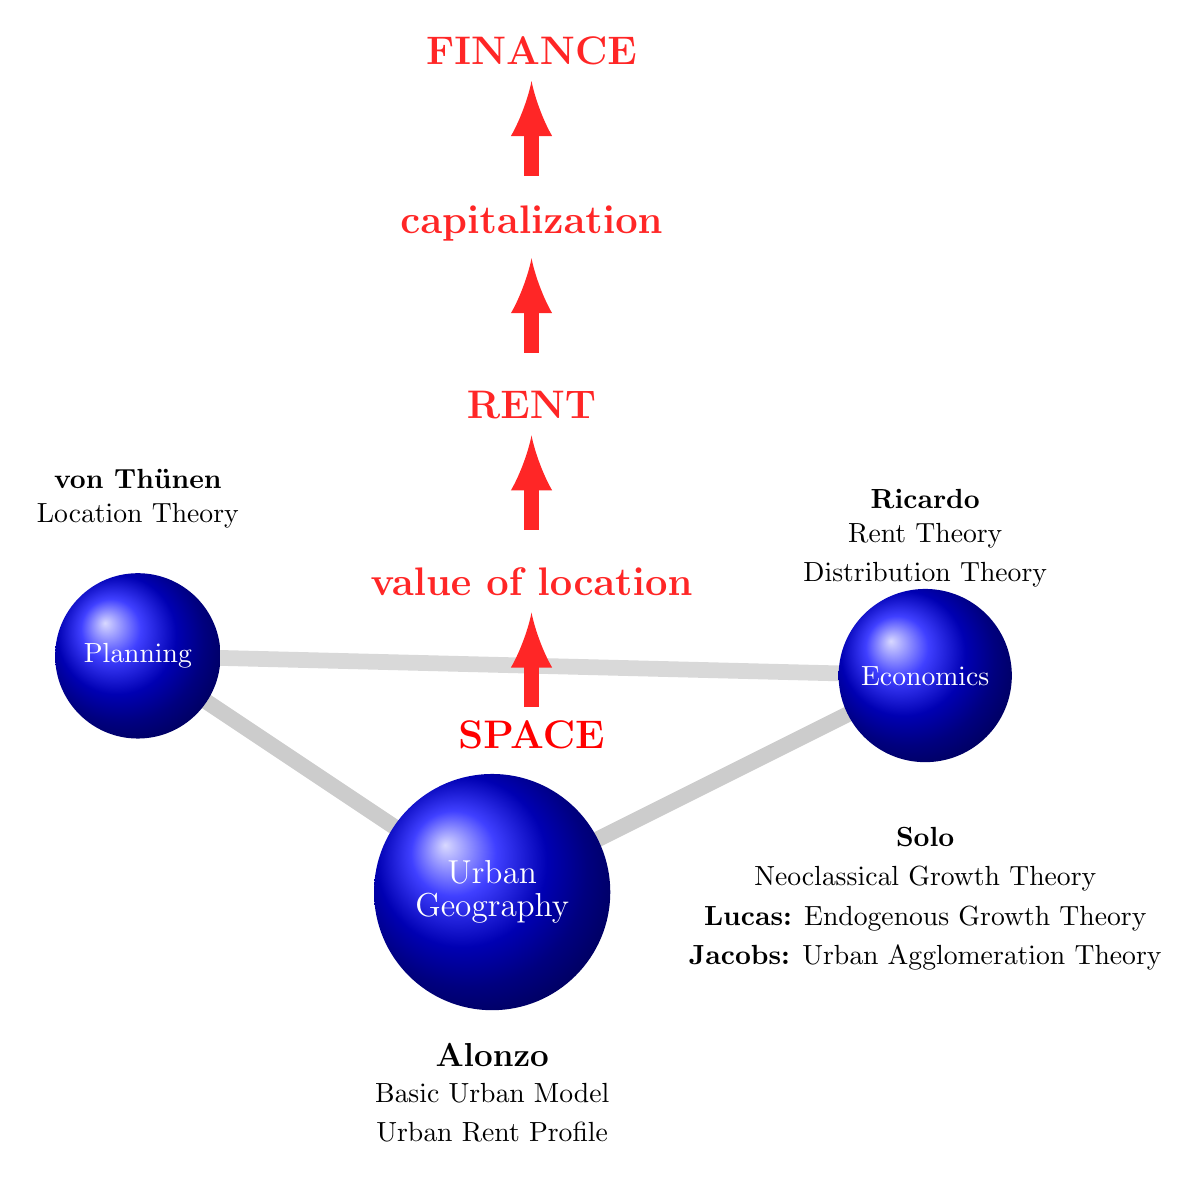
\begin{tikzpicture}{scale=.5}
% find color cotrol for ball. Tind way to stop line short of node
\coordinate (planning) at (-5,1);%PREFACE
\coordinate (economics) at (5,.75);%
 \coordinate (geography) at (-.5,-2); %history
\coordinate (finance) at (0,5); %

\draw [line width=2mm, black!15, ] (planning)--(economics);
\draw [line width=2mm, black!20, ] (geography)--(economics);
\draw [line width=2mm, black!20, ] (geography)--(planning);

%\draw [line width=2mm, black!25, ] (geography)--(finance);
%\draw [line width=2mm, black!20, ] (planning)--(finance);
%\draw [line width=2mm, black!20, ] (finance)--(economics);

\node [circle,shading=ball, minimum width=2.1   cm, white, align=center] (ball) at (planning) {Planning};
\node [circle,shading=ball, minimum width=2.2cm, white, align=center] (ball) at (economics) {Economics};
\node [circle,shading=ball, minimum width=3cm, white, align=center] (ball) at (geography)[text width=2cm] {\large Urban\\ Geography};

%\node [circle, shading=ball, minimum width=2.4cm, white, align=center] (ball) at (finance)[text width=2cm] {Finance};

%\node at (-.3,-.1) [red] {\Large \textbf{RENT}};

% new stuff
\node at (planning) [above=2cm] {\textbf{von Th\"unen}};
\node at (planning) [above=1.5cm] {Location Theory};

\node at (economics) [above=2cm] {\textbf{Ricardo}};
\node at (economics) [above=1.5cm] {Rent Theory};
\node at (economics) [above=1.0cm] {Distribution Theory};

\node at (economics) [below=1.8cm] {\textbf{Solo}};
\node at (economics) [below=2.3cm] {Neoclassical Growth Theory};
\node at (economics) [below=2.8cm] {\textbf{Lucas:} Endogenous Growth Theory};
\node at (economics) [below=3.3cm] {\textbf{Jacobs:} Urban Agglomeration Theory};


\node at (geography) [below=1.8cm] {\textbf{\large Alonzo}};
\node at (geography) [below=2.3cm] {Basic Urban Model};
\node at (geography) [below=2.8cm] {Urban Rent Profile};

%\node [circle, shading=ball, minimum width=2.4cm, white, align=center] (ball) at (finance)[text width=2cm] {Finance};
\draw [line width=2mm, red!85, -latex ] (0, 7.1)--++(0,1.2)node[above=-.1] {\Large \textbf{FINANCE}};
\draw [line width=2mm, red!85, -latex ] (0, 4.85)--++(0,1.2)node[above=-.1] {\Large \textbf{capitalization}};
\draw [line width=2mm, red!85, -latex ] (0, 2.6)--++(0,1.2)node[above=-.1] {\Large \textbf{RENT}};
\draw [line width=2mm, red!85, -latex ] (0, .35)--++(0,1.2)node[above=-.1] {\Large \textbf{value of location}};
\node at (0,0) [red] {\Large \textbf{SPACE}};


\end{tikzpicture}

    \caption{space and value}
    \label{fig-space-value}
\end{figure}

Land rent was historically the basis of the wealth and political power of  the land-owning class in the era of the classical economists. % #E NEED MORE HERE


We further link the model of urban rents to emerging concerns about the financialization of the housing market. The key insight we offer is that the financialization  of the housing sector is a  form of rent-seeking that must have detrimental effects on urban development and on the well-being of urban residents.


% #E NEED TO POSITION THIS WORK IN RELATION TO THE MARGINALIST ACCOUNT IN THIS SECTION BECAUSE IT IS ONE OF THE FEW THINGS YOU HAVE INTRODUCES. tHE URBAN MODELS YOU DESCRIBE HERE SHOULD BE FRAMED BY WHAT YOU ADD IN BACKGROUND ABOUT PLANNING/URBAN MODELS (AS PER MY SUGGESTION IN THAT SECTION) 
% #E YOU ALSO NEED TO ADD A SUMMARIZING PARAGRAPH WHICH I CAN HELP WRITE WHEN THIS SECTION IS MORE FILLED OUT. MAYBE THIS:
% #E ADD: By bringing these approaches into a coherent approach, we can better account for  WHAT... EXPLAIN THAT alone they don't give as complete a picture. This thesis show that certain things become clear when they are brought together that provide an better account of the current situation. Older economics models do not predict certain things that are currently happening. This is because they are based on out of date modes of production, fail to account for the importance of location value and the modelling tools available when they were developed required some simplification.   Updating the models for the changing times, using more complex modelling systems and incorporating space with the economic models allow us to create models and narratives that provide a more effective understanding of the situation as it stands today. 





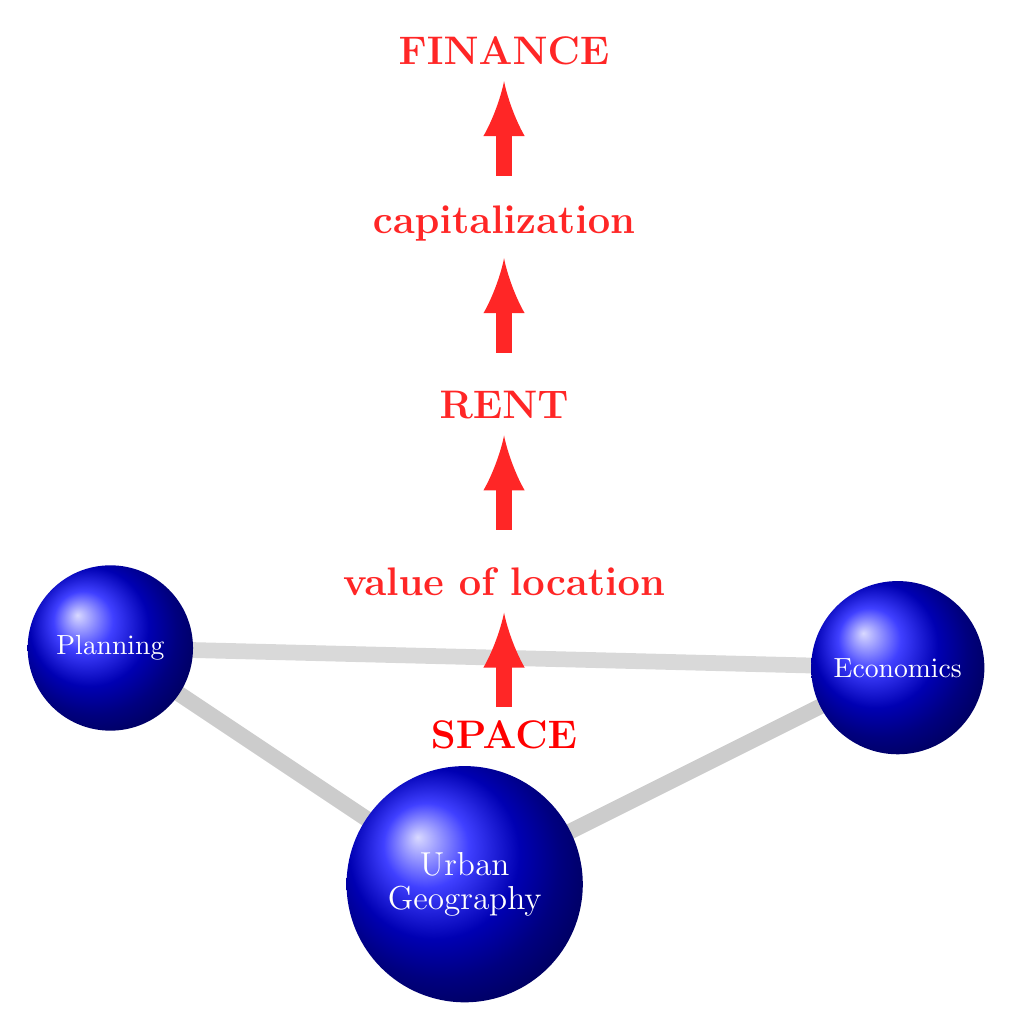
\begin{tikzpicture}{scale=.5}
% find color cotrol for ball. Tind way to stop line short of node
\coordinate (planning) at (-5,1);%PREFACE
\coordinate (economics) at (5,.75);%
 \coordinate (geography) at (-.5,-2); %history
\coordinate (finance) at (0,5); %

\draw [line width=2mm, black!15, ] (planning)--(economics);
\draw [line width=2mm, black!20, ] (geography)--(economics);
\draw [line width=2mm, black!20, ] (geography)--(planning);

%\draw [line width=2mm, black!25, ] (geography)--(finance);
%\draw [line width=2mm, black!20, ] (planning)--(finance);
%\draw [line width=2mm, black!20, ] (finance)--(economics);

\node [circle,shading=ball, minimum width=2.1   cm, white, align=center] (ball) at (planning) {Planning};
\node [circle,shading=ball, minimum width=2.2cm, white, align=center] (ball) at (economics) {Economics};
\node [circle,shading=ball, minimum width=3cm, white, align=center] (ball) at (geography)[text width=2cm] {\large Urban\\ Geography};

%\node [circle, shading=ball, minimum width=2.4cm, white, align=center] (ball) at (finance)[text width=2cm] {Finance};
\draw [line width=2mm, red!85, -latex ] (0, 7)--++(0,1.2)node[above=-.1] {\Large \textbf{FINANCE}};
\draw [line width=2mm, red!85, -latex ] (0, 4.75)--++(0,1.2)node[above=-.1] {\Large \textbf{capitalization}};
\draw [line width=2mm, red!85, -latex ] (0, 2.5)--++(0,1.2)node[above=-.1] {\Large \textbf{RENT}};
\draw [line width=2mm, red!85, -latex ] (0, .25)--++(0,1.2)node[above=-.1] {\Large \textbf{value of location}};
\node at (0,-.1) [red] {\Large \textbf{SPACE}};
\end{tikzpicture}



% \vspace {2cm}
% Figure 4 with finance

% \begin{tikzpicture}{scale=.5}
% % find color cotrol for ball. Tind way to stop line short of node
% \coordinate (planning) at (-5,1);%PREFACE
% \coordinate (economics) at (5,.75);%
%  \coordinate (geography) at (-.5,-2); %history
% \coordinate (finance) at (0,5); %

% \draw [line width=2mm, black!15, ] (planning)--(economics);
% \draw [line width=2mm, black!20, ] (geography)--(economics);
% \draw [line width=2mm, black!20, ] (geography)--(planning);

% \node at (-.3,2) [red] {\huge \textbf{RENT}};

% \draw [line width=3mm,  black!50,opacity=.5 ] (geography)--(finance);
% \draw [line width=2mm, black!20, ] (planning)--(finance);
% \draw [line width=2mm, black!20, ] (finance)--(economics);

% \node [circle,shading=ball, minimum width=2.1   cm, white, align=center] (ball) at (planning) {Planning};
% \node [circle,shading=ball, minimum width=2.2cm, white, align=center] (ball) at (economics) {Economics};
% \node [circle,shading=ball, minimum width=3 . cm, white, align=center] (ball) at (geography)[text width=2cm] {\large Urban\\ Geography};

% \node [circle, shading=ball, minimum width=2.4cm, white, align=center] (ball) at (finance)[text width=2cm] {Finance};


% \end{tikzpicture}



\vspace {2cm}
Figure 4 with finance

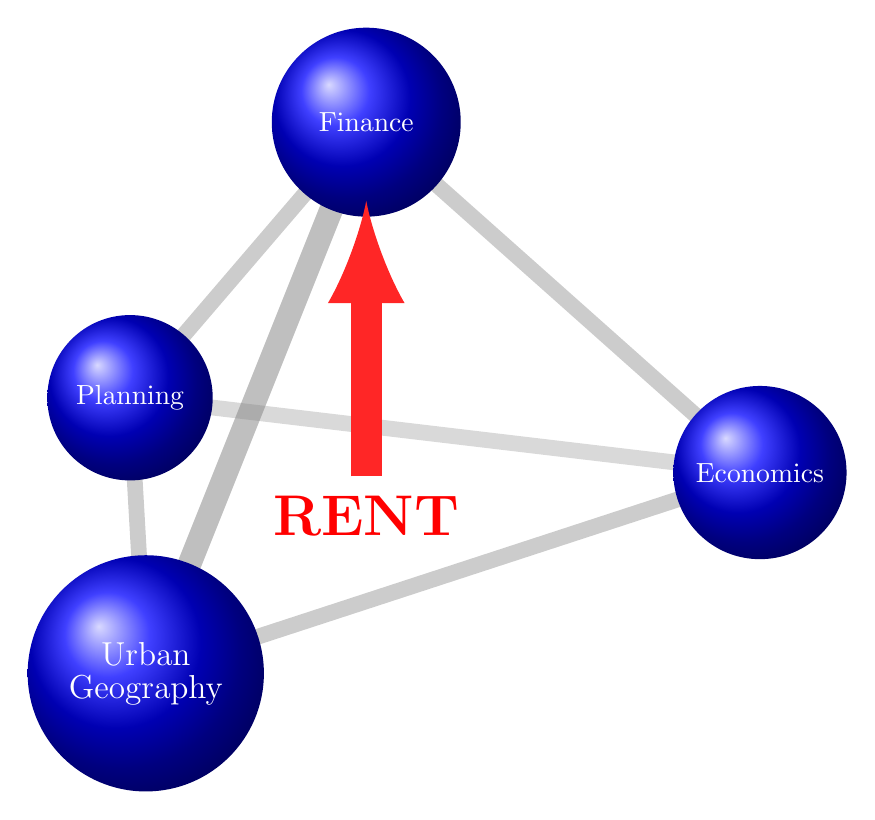
\begin{tikzpicture}{scale=.5}
% find color cotrol for ball. Tind way to stop line short of node
\coordinate (planning) at (-3,1.5);%PREFACE
\coordinate (economics) at (5,.55);%
 \coordinate (geography) at (-2.8,-2); %history
\coordinate (finance) at (0,5); %

\draw [line width=2mm, black!15, ] (planning)--(economics);
\draw [line width=2mm, black!20, ] (geography)--(economics);
\draw [line width=2mm, black!20, ] (geography)--(planning);

\node at (.0,0) [red] {\huge \textbf{RENT}};

\draw [line width=3mm,  black!50,opacity=.5 ] (geography)--(finance);
\draw [line width=2mm, black!20, ] (planning)--(finance);
\draw [line width=2mm, black!20, ] (finance)--(economics);

\node [circle,shading=ball, minimum width=2.1   cm, white, align=center] (ball) at (planning) {Planning};
\node [circle,shading=ball, minimum width=2.2cm, white, align=center] (ball) at (economics) {Economics};
\node [circle,shading=ball, minimum width=3cm, white, align=center] (ball) at (geography)[text width=2cm] {\large Urban\\ Geography};

\node [circle, shading=ball, minimum width=2.4cm, white, align=center] (ball) at (finance)[text width=2cm] {Finance};
\draw [line width=4mm, red!85, -latex ] (0, .5)--(0,4);


\end{tikzpicture}



